\newpage

\section*{Author Contributions}
This work was an open-source collaborative effort across multiple institutions. We employed a point-based system to determine contributions and award authorships, with technical contributions tracked and measured in units of pull requests (PRs)\footnote{For more details, please refer to \url{https://github.com/All-Hands-AI/OpenHands/pull/1917}.}. Xingyao Wang led the project, coordinating overall development and paper writing efforts. Detailed contributions were as follows:

\begin{itemize}[noitemsep,topsep=0pt,parsep=2pt,partopsep=0pt,leftmargin=18pt]

\item \textbf{Agent Development} (\sref{sec:agenthub}): Xingyao Wang led the implementation of CodeAct \cite{wang2024executable} and CodeActSWE agents. Frank F. Xu led the development of web browsing agents \cite{zhou2023webarena}. Mingchen Zhuge orchestrated the integration of the GPTSwarm agent \cite{zhuge2024language}. Robert Brennan and Boxuan Li lead the development of the Micro Agent.

\item \textbf{Architectural Development} (\fref{fig:arch}): Robert Brennan initiated the architecture design. Boxuan Li, Frank F. Xu, Xingyao Wang, Yufan Song, and Mingzhang Zheng further refined and expanded the architecture. Boxuan Li implemented the initial version of integration tests (\sref{sec:integration-tests}), maintained the agentskills library (\sref{sec:agent-skills}), managed configurations, and resolved resource leaks in evaluation. Frank F. Xu developed the web browsing environment (\sref{sec:browsergym-actions}) for both agent execution and evaluation and integrated it with both agent and front-end user interfaces. Xingyao Wang authored the initial code for the agentskills library and the Docker sandbox. Yufan Song implemented cost tracking for evaluation, while Mingzhang Zheng developed an image-agnostic docker sandbox for more stable SWE-Bench evaluation.

\item \textbf{Benchmarking, Integration, and Code Review}: Boxuan Li and Yufan Song led benchmark integration efforts, including coordination, evaluation, and code review. Yufan Song also helped track PR contributions. Graham Neubig, Xingyao Wang, Mingzhang Zheng, Robert Brennan, Hoang H. Tran, Frank F. Xu, Xiangru Tang, Fuqiang Li, and Yanjun Shao provided additional support in integration and code reviews.
Specific benchmark contributions included:
\begin{itemize}
    \item SWE-Bench \cite{jimenez2024swebench}: Bowen Li and Xingyao Wang
    \item WebArena \cite{zhou2023webarena} and MiniWob++ \cite{liu2018reinforcement}: Frank F. Xu
    \item GAIA \cite{gaia}: Jiayi Pan (integration) and Mingchen Zhuge (GPTSwarm evaluation)
    \item API-Bench \cite{patil2023gorilla} and ToolQA \cite{zhuang2024toolqa}: Yueqi Song
    \item HumanEvalFix \cite{muennighoff2024octopack}: Niklas Muennighoff and Xiangru Tang
    \item ProofWriter \cite{proofwriter}: Ren Ma
    \item MINT \cite{wang2024mint}: Hoang H. Tran
    \item AgentBench \cite{liu2023agentbench}: Fuqiang Li
    \item BIRD \cite{bird}: Binyuan Hui
    \item GPQA \cite{rein2023gpqa}: Jaskirat Singh
    \item BioCoder \cite{tang2023biocoder}: Xiangru Tang and Bill Qian
    \item ML-Bench \cite{liu2024mlbench}: Xiangru Tang and Yanjun Shao
    \item Entity-Deduction-Arena \cite{zhang2023entity}: Yizhe Zhang
\end{itemize}

\item \textbf{Advising}: Graham Neubig advised the project, providing guidance, resources, and substantial paper edits. Heng Ji and Hao Peng offered additional project advice and assisted with paper writing. Junyang Lin contributed advisory support and sponsored resources.
\end{itemize}














\section{Limitations and Future Work}
\label{sec:limitation-future-work}
We are excited about the foundations our vibrant community has laid in \projname and look forward to its continued evolution.
We identify several directions for future work:

\textbf{Enhanced multi-modality support.} While our current implementation already supports a wide range of file formats through predefined agent skills, we are interested in enabling multi-modality in a principled way through standard IPython and browser integration, such as viewing images and videos using vision-language model through a browser or processing XLSX files with code.

\textbf{Stronger agents.} Current agents still struggle with complex tasks, and we are interested in building better agents through both training and inference time techniques. 

\textbf{Agent editing improvements.} Current agent suffers a lot when editing long files, and we are interested in exploring different approaches to improve the file editing performance of agents.

\textbf{Web browsing improvements.} Due to the extensible nature of \projname, orthogonal components that could improve agents can be integrated easily. For example, thanks to \projname's extensible architecture, Auto Eval \& Refine~\cite{pan2024autonomous}, an agent retry-on-error strategy with Reflexion~\cite{shinn2024reflexion} prompts and task completion reward models, will be integrated as an optional component attached to our browsing agent.



\textbf{Automatic workflow generation.} Currently, OpenHands's workflow still requires a substantial handcrafted workload. We believe that graph-based frameworks such as GPTSwarm~\cite{zhuge2024language} and LangGraph~\cite{langchain2022} could serve as alternative solutions for building agents. Particularly in GPTSwarm, when agents are constructed using graphs, it becomes easier to incorporate various optimization methods (e.g., reinforcement learning, meta-prompting). OpenHands considers these methods to lay the groundwork for promising solutions in automatic workflow generation in future versions.

\section{Ethics Statement}
\label{sec:ethics}
Most AI agents today are still research artifacts and lack the ability to perform complex, long-horizon tasks in the real world reliably. However, as their performance continues to improve and they are increasingly deployed in real world, they have the potential to boost productivity while also posing security risks to society significantly.
\projname helps mitigate risks by: 
\begin{itemize}[noitemsep,topsep=0pt,parsep=2pt,partopsep=0pt,leftmargin=18pt]
\item[(1)] Enabling systematic evaluation of these agents, which can identify and address risks before they are widely deployed.
\item[(2)] Facilitating human-agent interaction rather than allowing agents to operate autonomously without oversight.
\item[(3)] More importantly, we hope \projname allows researchers worldwide to access the best suites of agents to conduct frontier safety research towards building safe and helpful agents.
\end{itemize}



\section{Related Work}
\label{sec:related_work}

The breakthroughs in large language models (LLMs) like ChatGPT~\cite{openai2024chatgpt} and GPT-4~\cite{openai2024gpt4} have significantly enhanced the capabilities of autonomous agents across various domains~\cite{ye2023proagent,tang2024medagents,park2023generative,cui2023chatlaw}. These advances have spurred a multitude of generalist agent proposals~\cite{gravitasauto,nakajima2023task,wu2023autogen} aimed at performing diverse user tasks and have gained attention from both developers and broader audiences. Notable works such as Auto-GPT~\cite{gravitasauto} harness LLMs for task completion by decomposing user goals into executable steps. Multi-agent collaboration systems leverage LLMs for elements like role-playing and task-solving capabilities~\cite{zhuge2023mindstorms,li2023camel,zhou2023agents,xagent2023}, with MetaGPT~\cite{hong2023metagpt} emphasizing standardized operating procedures, and AutoGen~\cite{wu2023autogen} providing a conversation framework for interactive systems. AGENTS~\cite{zhou2023agents} and AutoAgents~\cite{chen2024autoagents} offer new paradigms for customizable agent architecture, while XAgent~\cite{xagent2023} and GPTSwarm~\cite{zhuge2024language} introduce complex management systems and optimizable graphs, respectively, for enhanced agent operations.

This surge in agent development has led to specialized frameworks aimed at streamlining agent implementation. LangChain and LangGraph \cite{langchain2022} provide foundational building blocks with basic runtime support, while CrewAI \cite{crewai2024} focuses on orchestrating multi-agent communications. BrowserGym \cite{browsergym} specifically targets web browsing capabilities, and DSPy \cite{khattab2024dspy} emphasizes end-to-end prompt optimization. AutoGen~\cite{wu2023autogen} advances beyond basic frameworks by implementing Python and bash execution capabilities, though with stateless command execution, while frameworks like CrewAI offer sandboxed but limited code interpreter features.

Software development, a front-runner in applying LLM-based agents, has seen advancements in frameworks for facilitating the development processes~\cite{hong2023metagpt,qian2023communicative}. Innovations such as ChatDev~\cite{qian2023communicative} automate the software development lifecycle akin to the waterfall model, and AutoCodeRover~\cite{zhang2024autocoderover} addresses GitHub issues via code search and abstract syntax tree manipulation. AgentCoder~\cite{huang2024agentcoder} iteratively refines code generation with integrated testing and feedback, while SWE-Agent~\cite{yang2024sweagent} integrates LLMs for automated Github issue fixing, streamlining software engineering.


\section{Graphical User Interface}
\label{sec:ui}

Besides running from the command line, \projname features a rich graphical user interface that visualizes the agent's current actions (\eg, browsing the web, executing base commands or Python code, \etc) and allows for real-time feedback from the user.
Screenshots of the UI are shown in \fref{fig:ui}.
The user may interrupt the agent at any moment to provide additional feedback, comments, or instruction while the agent is working.
This user interface directly connects with the event streams (\sref{sec:agent-abstraction}) to control and visualize the agents and runtime, making it agent and runtime agnostic.


\section{Quality Control: Integration Tests for Agents}
\label{sec:integration-tests}

Integration tests \cite{DBLP:conf/icsm/LeungW90} have long been used by software developers to ensure software quality. Unlike large language models with simple input-output schema, agents are typically complex pieces of software where minor errors can be easily introduced during the development process and hurt final task performance.
While running a full suite evaluation (\sref{sec:evaluation}) is the ultimate measure of performance degradation, running them for \textit{every} code changes can be prohibitively slow and expensive.
\footnote{Running a SWE-Bench Lite \cite{jimenez2024swebench} evaluation with \texttt{gpt-4o} costs around 600 USD.}.
In \projname, we pioneer an end-to-end agent test framework that tests prompt regression, actions, and sandbox environments.
It combines integration testing from software engineering and foundation model mocking for deterministic behavior to prevent the accidental introduction of bugs during agent development. 


\noindent \textbf{Defining an integration test.}
The integration test framework for OpenHands is structured to validate end-to-end functionality by automating task execution and result verification. Developers define tasks and expected results; for instance, a task might involve correcting typos in a document named "bad.txt". Upon task execution through OpenHands, outputs are compared against a predefined "gold file" to ensure accuracy.

\noindent \textbf{Mocking LLM for deterministic behavior.}
Addressing the challenge of non-determinism in large language models (LLMs) and the associated high costs, the framework intercepts all LLM calls and supplies predefined responses based on exact prompt matches. This method not only ensures consistency in test outcomes but also reduces operational costs by minimizing the reliance on real LLMs.

\noindent \textbf{Regenerate LLM responses on breaking changes.}
Prompt-response pairs are managed through a script that generates and stores these pairs when new tests are introduced or existing prompts are modified. For routine tests, the framework attempts to reuse existing LLM responses by slightly adjusting the prompts. Substantial changes that affect task handling require regeneration of these pairs using real LLMs.

\noindent \textbf{Benefits of integration tests.}
The framework offers several advantages, including 1) Prompt regression testing: Stored prompt-response pairs facilitate change tracking and provide a reference for new team members to understand LLM interactions, 2) Multi-platform support: Tests are automatically scheduled for every pull request and commit on the main branch, running across multiple platforms, environments, and agents, including Linux and Mac, and in local, SSH, and exec sandboxes, and 3) Comprehensive error detection: It captures errors in prompt generation, message passing, and sandbox execution, thereby maintaining a high test coverage.

\section{How \projname Runtime work}
\label{sec:runtime-details}

\subsection{Workflow}
The OpenHands Runtime system uses a client-server architecture implemented with Docker containers. See \fref{fig:runtime_workflow} for an overview of how it works.

\begin{figure}
\centering
\vspace{-0.2cm}
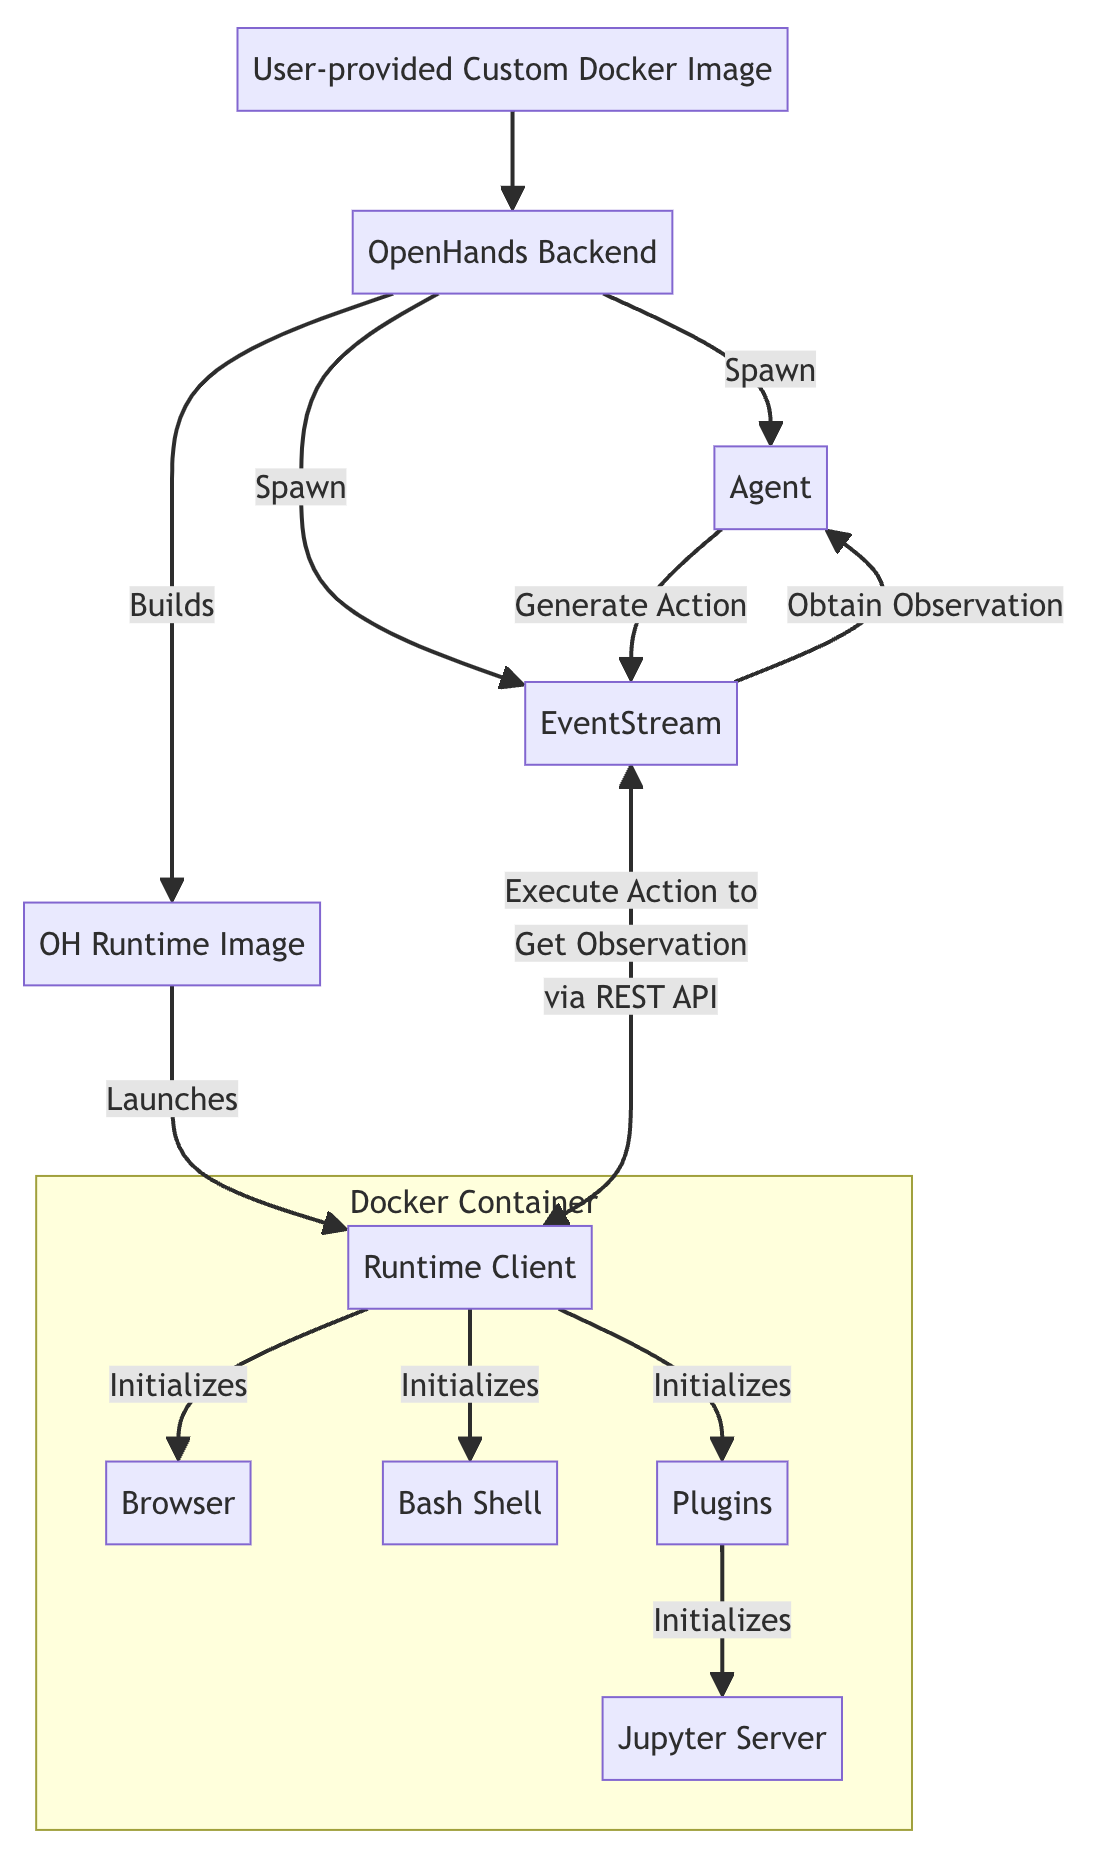
\includegraphics[height=0.8\textwidth]{figs/runtime/oh_runtime_workflow.png}
\vspace{-0.2cm}
\caption{\projname runtime workflow.}
\label{fig:runtime_workflow}
\vskip -0.1in
\end{figure}

\begin{itemize}[noitemsep,topsep=0pt,parsep=2pt,partopsep=0pt,leftmargin=18pt]
\item[(1)] \textbf{User Input}: The user provides a custom base Docker image.

\item[(2)] \textbf{Image Building}: OpenHands builds a new Docker image (the "OH runtime image") based on the user-provided image. This new image includes OpenHands-specific code, primarily the "runtime client" (i.e., runtime API server described in \sref{sec:agent-runtime}).
\item[(3)] \textbf{Container Launch}: When OpenHands starts, it launches a Docker container using the OH runtime image.
\item[(4)] \textbf{Communication}: The OpenHands backend (\texttt{runtime.py}) communicates with the runtime client over RESTful API, sending actions and receiving observations
\item[(5)] \textbf{Action Execution}: The runtime client receives actions from the backend, executes them in the sandboxed environment, and sends back observations

\item[(6)] \textbf{Observation Return}: The client sends execution results back to the OpenHands backend event stream as observations.

\end{itemize}

The role of the client:
\begin{itemize}
    \item It acts as an intermediary between the OpenHands backend and the sandboxed environment
    \item It executes various types of actions (shell commands, file operations, Python code, etc.) safely within the container
    \item It manages the state of the sandboxed environment, including the current working directory and loaded plugins
    \item It formats and returns observations to the backend, ensuring a consistent interface for processing results
\end{itemize}


\subsection{How OpenHands builds and maintains runtime images}

OpenHands' approach to building and managing runtime images ensures efficiency, consistency, and flexibility in creating and maintaining Docker images for both production and development environments.


\subsubsection{Image Tagging System}

OpenHands uses a dual-tagging system for its runtime images to balance reproducibility with flexibility:

\begin{itemize}[noitemsep,topsep=0pt,parsep=2pt,partopsep=0pt,leftmargin=18pt]
\item[(1)] Hash-based tag: \texttt{\{target\_image\_repo\}:\{target\_image\_hash\_tag\}}.
   Example: \texttt{runtime:abc123def456}
    \begin{itemize}
        \item This tag is based on the MD5 hash of the Docker build folder, which includes the source code (of runtime client and related dependencies) and Dockerfile
        \item Identical hash tags guarantee that the images were built with exactly the same source code and Dockerfile
        \item This ensures reproducibility; the same hash always means the same image contents
    \end{itemize}

\item[(2)] Generic tag: \texttt{\{target\_image\_repo\}:\{target\_image\_tag\}}.
   Example: \texttt{runtime:oh\_v0.9.3\_ubuntu\_tag\_22.04}

   \begin{itemize}
       \item This tag follows the format: \texttt{runtime:oh\_v\{VERSION\}\_\{BASE\_IMAGE\}\_tag\_\{IMAGE\_TAG\}}
       \item It represents the latest build for a particular base image and OpenHands version combination
       \item This tag is updated whenever a new image is built from the same base image, even if the source code changes
   \end{itemize}
\end{itemize}

The hash-based tag ensures reproducibility, while the generic tag provides a stable reference to the latest version of a particular configuration. This dual-tagging approach allows OpenHands to efficiently manage both development and production environments.

\subsubsection{Build Process}

\begin{itemize}[noitemsep,topsep=0pt,parsep=2pt,partopsep=0pt,leftmargin=18pt]
\item[(1)] \textbf{Image Naming Convention}:
    \begin{itemize}
    \item Hash-based tag: \texttt{{target\_image\_repo}:{target\_image\_hash\_tag}}.
     Example: \texttt{runtime:abc123def456}
     \item Generic tag: \texttt{{target\_image\_repo}:{target\_image\_tag}}.
     Example: \texttt{runtime:oh\_v0.9.3\_ubuntu\_tag\_22.04}
    \end{itemize}

\item[(2)] \textbf{Build Process}:
   \begin{itemize}
   \item[a.] Convert the base image name to an OH runtime image name
      Example: \texttt{ubuntu:22.04} -> \texttt{runtime:oh\_v0.9.3\_ubuntu\_tag\_22.04}
   \item[b.] Generate a build context (Dockerfile and OpenHands source code) and calculate its hash
   \item[c.] Check for an existing image with the calculated hash
   \item[d.] If not found, check for a recent compatible image to use as a base
   \item[e.] If no compatible image exists, build from scratch using the original base image
   \item[f.] Tag the new image with both hash-based and generic tags
   \end{itemize}

\item[(3)] \textbf{Image Reuse and Rebuilding Logic}:
   The system follows these steps to determine whether to build a new image or use an existing one from a user-provided (base) image (e.g., \texttt{ubuntu:22.04}):
   \begin{itemize}
       \item[a.] If an image exists with the same hash (e.g., \texttt{runtime:abc123def456}), it will be reused as is
       \item[b.] If the exact hash is not found, the system will try to rebuild using the latest generic image (e.g., \texttt{runtime:oh\_v0.9.3\_ubuntu\_tag\_22.04}) as a base. This saves time by leveraging existing dependencies
       \item[c.] If neither the hash-tagged nor the generic-tagged image is found, the system will build the image completely from scratch
   \end{itemize}

\end{itemize}


\textbf{Caching and Efficiency.} The system attempts to reuse existing images when possible to save build time. If an exact match (by hash) is found, it's used without rebuilding. If a compatible image is found, it's used as a base for rebuilding, saving time on dependency installation.

A flowchart illustrating the build process is shown in \fref{fig:runtime-image-build-workflow}

\begin{figure}
\centering
\vspace{-0.2cm}
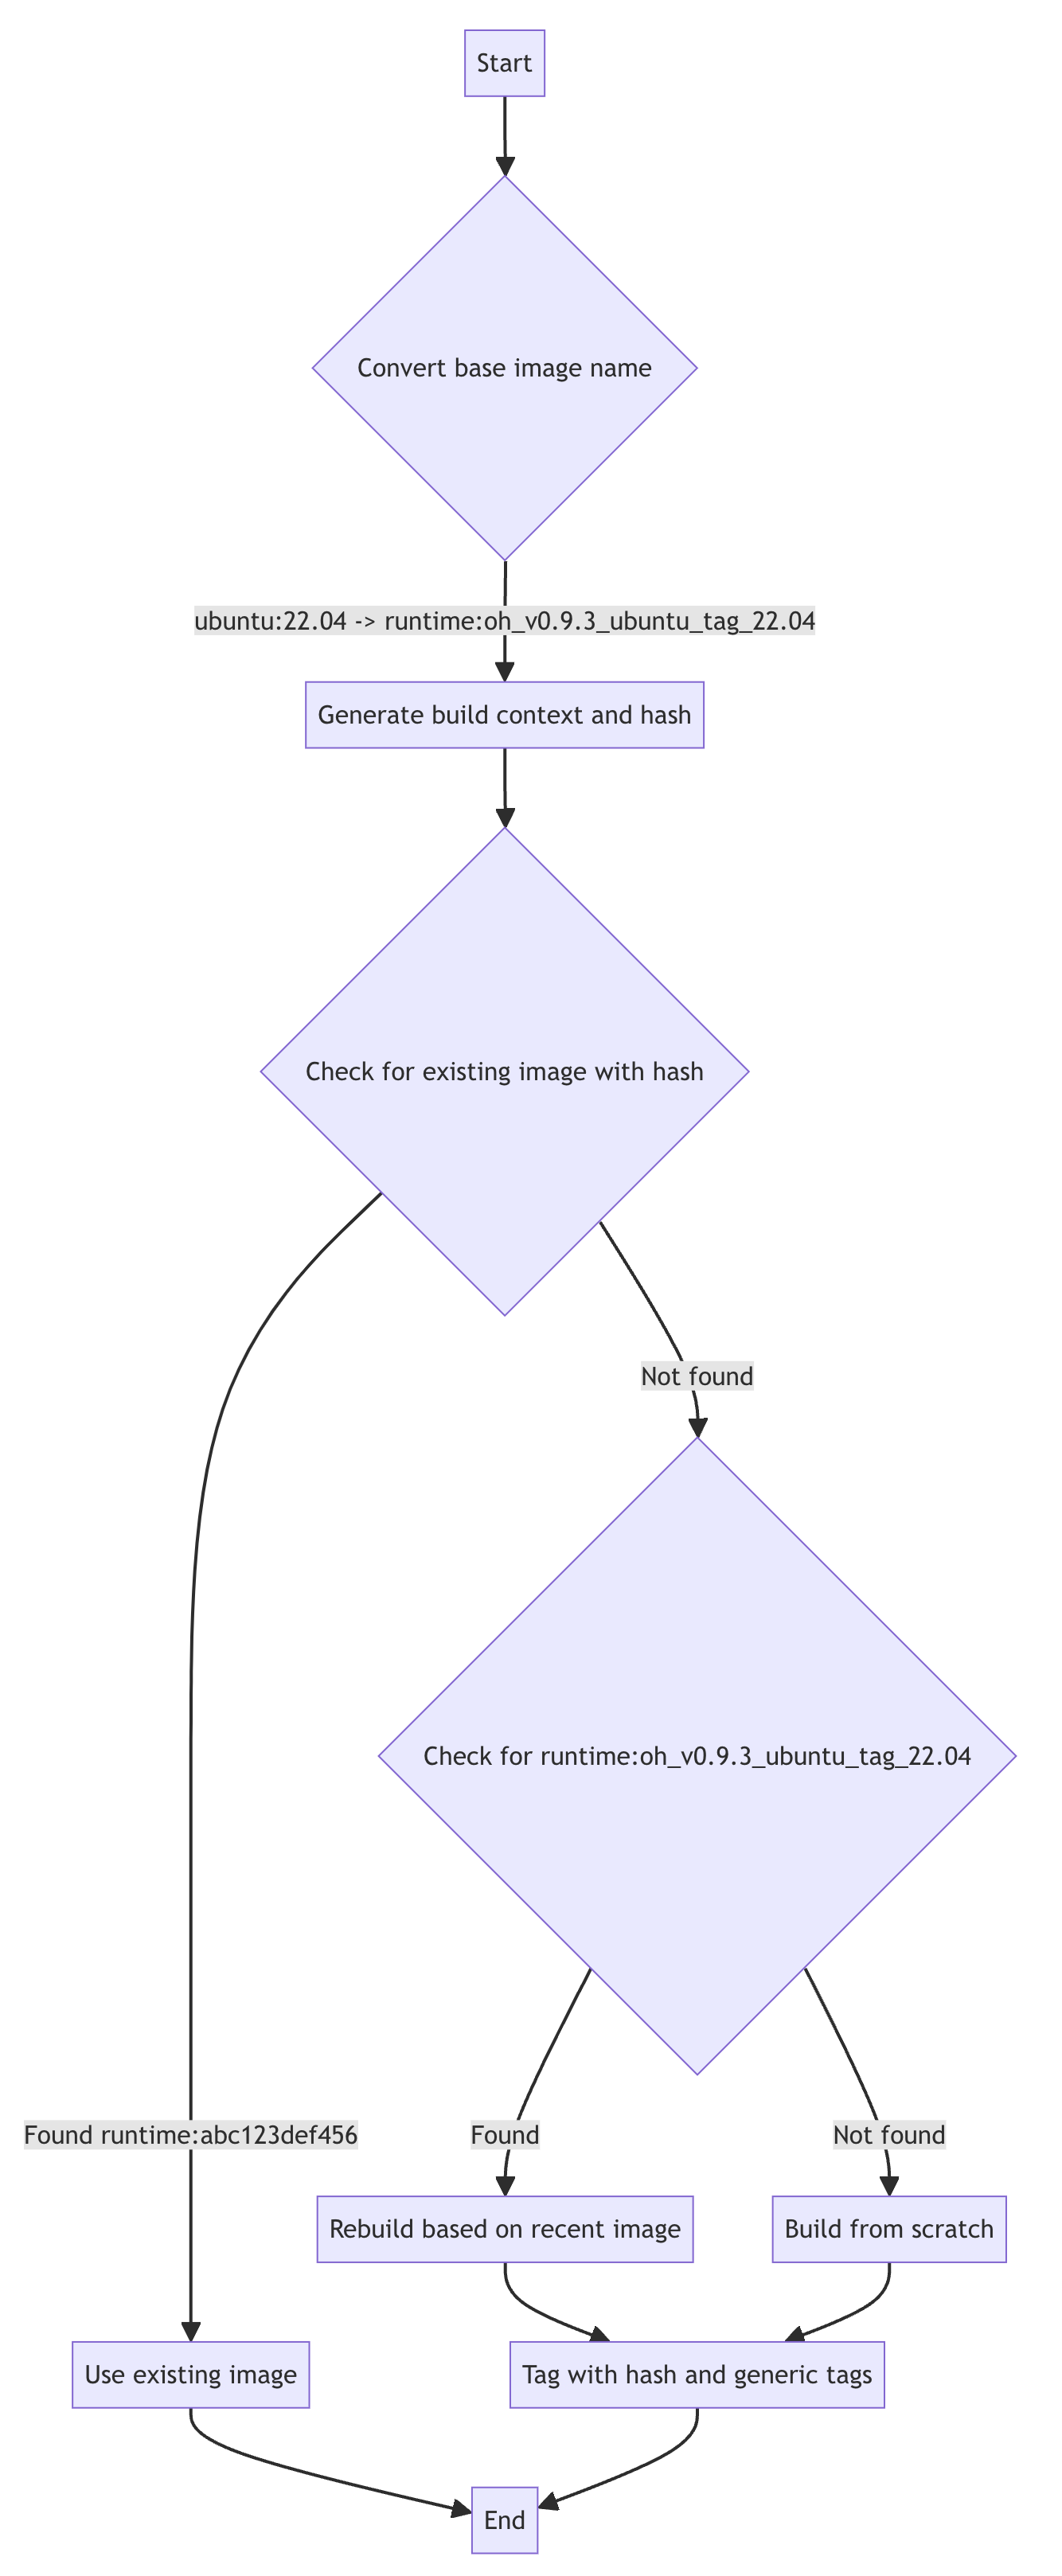
\includegraphics[width=0.5\textwidth]{figs/runtime/oh_runtime_image_build_workflow.png}
\vspace{-0.2cm}
\caption{\projname Runtime Image Build Workflow.}
\label{fig:runtime-image-build-workflow}
\vskip -0.1in
\end{figure}

\section{Additional Results For GPQA Benchmark}
\label{sec:gpqa-additional}

We showcase more detailed results, including performance on other subsets for GPQA benchmark in~\tref{tab:gpqa}.

\begin{table}[ht]
    \centering
    \small
    \caption{\emph{Full Evaluation Results on the GPQA Benchmark \cite{rein2023gpqa}} (\sref{sec:eval_misc_assistance}).
    }
\begin{adjustbox}{max width=\textwidth}
    \begin{tabular}{lcccc}
        \toprule
        \multirow{2}{*}{\textbf{Evaluation Method and Model}}  & \multicolumn{3}{c}{\textbf{Accuracy by subset (\%)}} & \multirow{2}{*}{\textbf{Avg Cost (\$)}} \\[0.5ex]
        
         & {\emph{Diamond Set}} & {\emph{Main Set}} & {\emph{Extended Set}} & \\ 
         \midrule
         \rowcolor{Gray} Expert Human Validators & 81.2 & 72.5 & 65.4 & N/A \\
        \rowcolor{Gray} Non-Expert Human Validators & 21.9 & 30.5 & 33.9 & N/A \\
        \midrule
        Few-Shot CoT Llama-2-70B-chat & 28.1 & 29.1 & 30.4 & \cellcolor{Gray}N/A \\ 
        Few-Shot CoT GPT-3.5-turbo-16k & 29.6 & 28.0 & 28.2 & \cellcolor{Gray}N/A \\ 
        Few-Shot CoT GPT-4 & 38.8 & 39.7 & 38.7 & \cellcolor{Gray}N/A \\ 
        GPT-4 with search (backoff to CoT on abstention) &  38.8 &  41.0 & 39.4 & \cellcolor{Gray}N/A \\
        \midrule
        OpenHands + CodeActAgent v1.5 + GPT3.5-turbo & 27.9 & 23.4 & 26.1 & 0.012 \\
        OpenHands + CodeActAgent v1.5 + GPT4-turbo & 51.8 & 47.4 & 42.4 & 0.501 \\
        OpenHands + CodeActAgent v1.5 + GPT4o & \textbf{53.1} &  \textbf{49.3} & \textbf{52.8} & 0.054 \\
        \bottomrule
    \end{tabular}
    \label{tab:gpqa}
\end{adjustbox}
\end{table}



\section{In-context Demonstration for CodeActSWEAgent}
\label{sec:icl-codeactswe}

The prompt is re-adopted from the SWE-agent's released trajectory (\url{https://github.com/princeton-nlp/SWE-agent/tree/main/trajectories/demonstrations}). The prompt can be found at \url{https://github.com/All-Hands-AI/OpenHands/blob/main/agenthub/codeact_swe_agent/prompt.py}.


\section{Supported AgentSkills}
\label{sec:supported-agentskills}

As of \projname v0.6, we support the following list of skills.
Please refer to the source code for the most up-to-date list of skills: \url{https://github.com/All-Hands-AI/OpenHands/blob/main/OpenHands/runtime/plugins/agent_skills/agentskills.py}


\begin{minted}[breaklines]{python}
def open_file(path: str, line_number: Optional[int] = None) -> None:
    """
    Opens the file at the given path in the editor. If line_number is provided, the window will be moved to include that line.

    Args:
        path: str: The path to the file to open.
        line_number: Optional[int]: The line number to move to.
    """
    pass


def goto_line(line_number: int) -> None:
    """
    Moves the window to show the specified line number.

    Args:
        line_number: int: The line number to move to.
    """
    pass

def scroll_down() -> None:
    """Moves the window down by 100 lines.

    Args:
        None
    """
    pass

def scroll_up() -> None:
    """Moves the window up by 100 lines.

    Args:
        None
    """
    pass

def create_file(filename: str) -> None:
    """Creates and opens a new file with the given name.

    Args:
        filename: str: The name of the file to create.
    """
    pass

def edit_file(start: int, end: int, content: str) -> None:
    """Edit a file.

    It replaces lines `start` through `end` (inclusive) with the given text `content` in the open file. Remember, the file must be open before editing.

    Args:
        start: int: The start line number. Must satisfy start >= 1.
        end: int: The end line number. Must satisfy start <= end <= number of lines in the file.
        content: str: The content to replace the lines with.
    """
    pass

def search_dir(search_term: str, dir_path: str = './') -> None:
    """Searches for search_term in all files in dir. If dir is not provided, searches in the current directory.

    Args:
        search_term: str: The term to search for.
        dir_path: Optional[str]: The path to the directory to search.
    """
    pass

def search_file(search_term: str, file_path: Optional[str] = None) -> None:
    """Searches for search_term in file. If file is not provided, searches in the current open file.

    Args:
        search_term: str: The term to search for.
        file_path: Optional[str]: The path to the file to search.
    """
    pass

def find_file(file_name: str, dir_path: str = './') -> None:
    """Finds all files with the given name in the specified directory.

    Args:
        file_name: str: The name of the file to find.
        dir_path: Optional[str]: The path to the directory to search.
    """
    pass

def parse_pdf(file_path: str) -> None:
    """Parses the content of a PDF file and prints it.

    Args:
        file_path: str: The path to the file to open.
    """
    pass

def parse_docx(file_path: str) -> None:
    """
    Parses the content of a DOCX file and prints it.

    Args:
        file_path: str: The path to the file to open.
    """
    pass

def parse_latex(file_path: str) -> None:
    """
    Parses the content of a LaTex file and prints it.

    Args:
        file_path: str: The path to the file to open.
    """
    pass

def parse_audio(file_path: str, model: str = 'whisper-1') -> None:
    """
    Parses the content of an audio file and prints it.

    Args:
        file_path: str: The path to the audio file to transcribe.
        model: Optional[str]: The audio model to use for transcription. Defaults to 'whisper-1'.
    """
    pass


def parse_image(
    file_path: str, task: str = 'Describe this image as detail as possible.'
) -> None:
    """
    Parses the content of an image file and prints the description.

    Args:
        file_path: str: The path to the file to open.
        task: Optional[str]: The task description for the API call. Defaults to 'Describe this image as detail as possible.'.
    """
    pass


def parse_video(
    file_path: str,
    task: str = 'Describe this image as detail as possible.',
    frame_interval: int = 30,
) -> None:
    """
    Parses the content of an image file and prints the description.

    Args:
        file_path: str: The path to the video file to open.
        task: Optional[str]: The task description for the API call. Defaults to 'Describe this image as detail as possible.'.
        frame_interval: Optional[int]: The interval between frames to analyze. Defaults to 30.

    """
    pass

def parse_pptx(file_path: str) -> None:
    """
    Parses the content of a pptx file and prints it.

    Args:
        file_path: str: The path to the file to open.
    """
    pass
\end{minted}


\section{BrowserGym Actions}
\label{sec:browsergym-actions}
The following are all the supported actions defined in BrowserGym\footnote{\url{https://github.com/ServiceNow/BrowserGym/blob/main/core/src/browsergym/core/action/functions.py}} as of v0.3.4.
The actions can be categorized into several types and can be configured to use only a subset of the functionality.
There are agent control actions, navigation actions, page element-based actions, coordinate-based actions, as well as tab-related actions.
We use these actions from the BrowserGym library as our main browsing action primitives.

\begin{minted}[breaklines]{python}
def send_msg_to_user(text: str):
    """
    Sends a message to the user.

    Examples:
        send_msg_to_user("Based on the results of my search, the city was built in 1751.")
    """
    pass

def report_infeasible(reason: str):
    """
    Notifies the user that their instructions are infeasible.

    Examples:
        report_infeasible("I cannot follow these instructions because there is no email field in this form.")
    """
    pass


def noop(wait_ms: float = 1000):
    """
    Do nothing, and optionally wait for the given time (in milliseconds).

    Examples:
        noop()
        noop(500)
    """
    pass


# https://playwright.dev/docs/input#text-input
def fill(bid: str, value: str):
    """
    Fill out a form field. It focuses the element and triggers an input event with the entered text.
    It works for <input>, <textarea> and [contenteditable] elements.

    Examples:
        fill('237', 'example value')
        fill('45', "multi-line\\nexample")
        fill('a12', "example with \\"quotes\\"")
    """
    pass


# https://playwright.dev/python/docs/api/class-locator#locator-check
def check(bid: str):
    """
    Ensure a checkbox or radio element is checked.

    Examples:
        check('55')
    """
    pass


# https://playwright.dev/python/docs/api/class-locator#locator-uncheck
def uncheck(bid: str):
    """
    Ensure a checkbox or radio element is unchecked.

    Examples:
        uncheck('a5289')
    """
    pass


# https://playwright.dev/docs/input#select-options
def select_option(bid: str, options: str | list[str]):
    """
    Select one or multiple options in a <select> element. You can specify
    option value or label to select. Multiple options can be selected.

    Examples:
        select_option('a48', "blue")
        select_option('c48', ["red", "green", "blue"])
    """
    pass


# https://playwright.dev/python/docs/api/class-locator#locator-click
def click(
    bid: str,
    button: Literal["left", "middle", "right"] = "left",
    modifiers: list[Literal["Alt", "Control", "Meta", "Shift"]] = [],
):
    """
    Click an element.

    Examples:
        click('a51')
        click('b22', button="right")
        click('48', button="middle", modifiers=["Shift"])
    """
    pass


# https://playwright.dev/python/docs/api/class-locator#locator-dblclick
def dblclick(
    bid: str,
    button: Literal["left", "middle", "right"] = "left",
    modifiers: list[Literal["Alt", "Control", "Meta", "Shift"]] = [],
):
    """
    Double click an element.

    Examples:
        dblclick('12')
        dblclick('ca42', button="right")
        dblclick('178', button="middle", modifiers=["Shift"])
    """
    pass


# https://playwright.dev/python/docs/api/class-locator#locator-hover
def hover(bid: str):
    """
    Hover over an element.

    Examples:
        hover('b8')
    """
    pass


# https://playwright.dev/python/docs/input#keys-and-shortcuts
def press(bid: str, key_comb: str):
    """
    Focus the matching element and press a combination of keys. It accepts
    the logical key names that are emitted in the keyboardEvent.key property
    of the keyboard events: Backquote, Minus, Equal, Backslash, Backspace,
    Tab, Delete, Escape, ArrowDown, End, Enter, Home, Insert, PageDown, PageUp,
    ArrowRight, ArrowUp, F1 - F12, Digit0 - Digit9, KeyA - KeyZ, etc. You can
    alternatively specify a single character you'd like to produce such as "a"
    or "#". Following modification shortcuts are also supported: Shift, Control,
    Alt, Meta.

    Examples:
        press('88', 'Backspace')
        press('a26', 'Control+a')
        press('a61', 'Meta+Shift+t')
    """
    pass


# https://playwright.dev/python/docs/api/class-locator#locator-focus
def focus(bid: str):
    """
    Focus the matching element.

    Examples:
        focus('b455')
    """
    pass


# https://playwright.dev/python/docs/api/class-locator#locator-clear
def clear(bid: str):
    """
    Clear the input field.

    Examples:
        clear('996')
    """
    pass


# https://playwright.dev/python/docs/input#drag-and-drop
def drag_and_drop(from_bid: str, to_bid: str):
    """
    Perform a drag & drop. Hover the element that will be dragged. Press
    left mouse button. Move mouse to the element that will receive the
    drop. Release left mouse button.

    Examples:
        drag_and_drop('56', '498')
    """
    pass


# https://playwright.dev/python/docs/api/class-mouse#mouse-wheel
def scroll(delta_x: float, delta_y: float):
    """
    Scroll horizontally and vertically. Amounts in pixels, positive for right or down scrolling, negative for left or up scrolling. Dispatches a wheel event.

    Examples:
        scroll(0, 200)
        scroll(-50.2, -100.5)
    """
    pass


# https://playwright.dev/python/docs/api/class-mouse#mouse-move
def mouse_move(x: float, y: float):
    """
    Move the mouse to a location. Uses absolute client coordinates in pixels.
    Dispatches a mousemove event.

    Examples:
        mouse_move(65.2, 158.5)
    """
    pass


# https://playwright.dev/python/docs/api/class-mouse#mouse-up
def mouse_up(x: float, y: float, button: Literal["left", "middle", "right"] = "left"):
    """
    Move the mouse to a location then release a mouse button. Dispatches
    mousemove and mouseup events.

    Examples:
        mouse_up(250, 120)
        mouse_up(47, 252, 'right')
    """
    pass


# https://playwright.dev/python/docs/api/class-mouse#mouse-down
def mouse_down(x: float, y: float, button: Literal["left", "middle", "right"] = "left"):
    """
    Move the mouse to a location then press and hold a mouse button. Dispatches
    mousemove and mousedown events.

    Examples:
        mouse_down(140.2, 580.1)
        mouse_down(458, 254.5, 'middle')
    """
    pass


# https://playwright.dev/python/docs/api/class-mouse#mouse-click
def mouse_click(x: float, y: float, button: Literal["left", "middle", "right"] = "left"):
    """
    Move the mouse to a location and click a mouse button. Dispatches mousemove,
    mousedown and mouseup events.

    Examples:
        mouse_click(887.2, 68)
        mouse_click(56, 712.56, 'right')
    """
    pass


# https://playwright.dev/python/docs/api/class-mouse#mouse-dblclick
def mouse_dblclick(x: float, y: float, button: Literal["left", "middle", "right"] = "left"):
    """
    Move the mouse to a location and double click a mouse button. Dispatches
    mousemove, mousedown and mouseup events.

    Examples:
        mouse_dblclick(5, 236)
        mouse_dblclick(87.5, 354, 'right')
    """
    pass


def mouse_drag_and_drop(from_x: float, from_y: float, to_x: float, to_y: float):
    """
    Drag and drop from a location to a location. Uses absolute client
    coordinates in pixels. Dispatches mousemove, mousedown and mouseup
    events.

    Examples:
        mouse_drag_and_drop(10.7, 325, 235.6, 24.54)
    """
    pass


# https://playwright.dev/python/docs/api/class-keyboard#keyboard-press
def keyboard_press(key: str):
    """
    Press a combination of keys. Accepts the logical key names that are
    emitted in the keyboardEvent.key property of the keyboard events:
    Backquote, Minus, Equal, Backslash, Backspace, Tab, Delete, Escape,
    ArrowDown, End, Enter, Home, Insert, PageDown, PageUp, ArrowRight,
    ArrowUp, F1 - F12, Digit0 - Digit9, KeyA - KeyZ, etc. You can
    alternatively specify a single character you'd like to produce such
    as "a" or "#". Following modification shortcuts are also supported:
    Shift, Control, Alt, Meta.

    Examples:
        keyboard_press('Backspace')
        keyboard_press('Control+a')
        keyboard_press('Meta+Shift+t')
        page.keyboard.press("PageDown")
    """
    pass


# https://playwright.dev/python/docs/api/class-keyboard#keyboard-up
def keyboard_up(key: str):
    """
    Release a keyboard key. Dispatches a keyup event. Accepts the logical
    key names that are emitted in the keyboardEvent.key property of the
    keyboard events: Backquote, Minus, Equal, Backslash, Backspace, Tab,
    Delete, Escape, ArrowDown, End, Enter, Home, Insert, PageDown, PageUp,
    ArrowRight, ArrowUp, F1 - F12, Digit0 - Digit9, KeyA - KeyZ, etc.
    You can alternatively specify a single character you'd like to produce
    such as "a" or "#".

    Examples:
        keyboard_up('Shift')
        keyboard_up('c')
    """
    pass


# https://playwright.dev/python/docs/api/class-keyboard#keyboard-down
def keyboard_down(key: str):
    """
    Press and holds a keyboard key. Dispatches a keydown event. Accepts the
    logical key names that are emitted in the keyboardEvent.key property of
    the keyboard events: Backquote, Minus, Equal, Backslash, Backspace, Tab,
    Delete, Escape, ArrowDown, End, Enter, Home, Insert, PageDown, PageUp,
    ArrowRight, ArrowUp, F1 - F12, Digit0 - Digit9, KeyA - KeyZ, etc. You can
    alternatively specify a single character such as "a" or "#".

    Examples:
        keyboard_up('Shift')
        keyboard_up('c')
    """
    pass


# https://playwright.dev/python/docs/api/class-keyboard#keyboard-type
def keyboard_type(text: str):
    """
    Types a string of text through the keyboard. Sends a keydown, keypress/input,
    and keyup event for each character in the text. Modifier keys DO NOT affect
    keyboard_type. Holding down Shift will not type the text in upper case.

    Examples:
        keyboard_type('Hello world!')
    """
    pass


# https://playwright.dev/python/docs/api/class-keyboard#keyboard-insert-text
def keyboard_insert_text(text: str):
    """
    Insert a string of text in the currently focused element. Dispatches only input
    event, does not emit the keydown, keyup or keypress events. Modifier keys DO NOT
    affect keyboard_insert_text. Holding down Shift will not type the text in upper
    case.

    Examples:
        keyboard_insert_text('Hello world!')
    """
    pass


# https://playwright.dev/python/docs/api/class-page#page-goto
def goto(url: str):
    """
    Navigate to a url.

    Examples:
        goto('http://www.example.com')
    """
    pass


# https://playwright.dev/python/docs/api/class-page#page-go-back
def go_back():
    """
    Navigate to the previous page in history.

    Examples:
        go_back()
    """
    pass


# https://playwright.dev/python/docs/api/class-page#page-go-forward
def go_forward():
    """
    Navigate to the next page in history.

    Examples:
        go_forward()
    """
    pass


# https://playwright.dev/python/docs/api/class-browsercontext#browser-context-new-page
def new_tab():
    """
    Open a new tab. It will become the active one.

    Examples:
        new_tab()
    """
    global page
    # set the new page as the active page
    page = page.context.new_page()
    # trigger the callback that sets this page as active in browsergym
    pass


# https://playwright.dev/python/docs/api/class-page#page-close
def tab_close():
    """
    Close the current tab.

    Examples:
        tab_close()
    """
    pass


# https://playwright.dev/python/docs/api/class-page#page-bring-to-front
def tab_focus(index: int):
    """
    Bring tab to front (activate tab).

    Examples:
        tab_focus(2)
    """
    pass


# https://playwright.dev/python/docs/input#upload-files
def upload_file(bid: str, file: str | list[str]):
    """
    Click an element and wait for a "filechooser" event, then select one
    or multiple input files for upload. Relative file paths are resolved
    relative to the current working directory. An empty list clears the
    selected files.

    Examples:
        upload_file("572", "my_receipt.pdf")
        upload_file("63", ["/home/bob/Documents/image.jpg", "/home/bob/Documents/file.zip"])
    """
    pass


# https://playwright.dev/python/docs/input#upload-files
def mouse_upload_file(x: float, y: float, file: str | list[str]):
    """
    Click a location and wait for a "filechooser" event, then select one
    or multiple input files for upload. Relative file paths are resolved
    relative to the current working directory. An empty list clears the
    selected files.

    Examples:
        mouse_upload_file(132.1, 547, "my_receipt.pdf")
        mouse_upload_file(328, 812, ["/home/bob/Documents/image.jpg", "/home/bob/Documents/file.zip"])
    """
    pass

\end{minted}

\section{Browsing Agent Details}
\label{sec:browsing-agent-details}

The following shows an example prompt containing all the information required for the current step to make a prediction about the next browsing actions.
Note that we also instruct the agent to predict multiple actions in one turn if the agent thinks they are meant to be executed sequentially without any feedback from the page.
This could save turns for common workflows that consist of a sequence of actions on the same page without any observation change, such as filling the username and password and submit in a login page.

\begin{minted}[breaklines]{text}
# Instructions
Review the current state of the page and all other information to find the best possible next action to accomplish your goal. Your answer will be interpreted and executed by a program, make sure to follow the formatting instructions.

# Goal:
Browse localhost:8000, and tell me the ultimate answer to life. Do not ask me for confirmation at any point.

# Action Space

16 different types of actions are available.

noop(wait_ms: float = 1000)
    Examples:
        noop()

        noop(500)

send_msg_to_user(text: str)
    Examples:
        send_msg_to_user('Based on the results of my search, the city was built in 1751.')

scroll(delta_x: float, delta_y: float)
    Examples:
        scroll(0, 200)

        scroll(-50.2, -100.5)

fill(bid: str, value: str)
    Examples:
        fill('237', 'example value')

        fill('45', 'multi-line\nexample')

        fill('a12', 'example with "quotes"')

select_option(bid: str, options: str | list[str])
    Examples:
        select_option('48', 'blue')

        select_option('48', ['red', 'green', 'blue'])

click(bid: str, button: Literal['left', 'middle', 'right'] = 'left', modifiers: list[typing.Literal['Alt', 'Control', 'Meta', 'Shift']] = [])
    Examples:
        click('51')

        click('b22', button='right')

        click('48', button='middle', modifiers=['Shift'])

dblclick(bid: str, button: Literal['left', 'middle', 'right'] = 'left', modifiers: list[typing.Literal['Alt', 'Control', 'Meta', 'Shift']] = [])
    Examples:
        dblclick('12')

        dblclick('ca42', button='right')

        dblclick('178', button='middle', modifiers=['Shift'])

hover(bid: str)
    Examples:
        hover('b8')

press(bid: str, key_comb: str)
    Examples:
        press('88', 'Backspace')

        press('a26', 'Control+a')

        press('a61', 'Meta+Shift+t')

focus(bid: str)
    Examples:
        focus('b455')

clear(bid: str)
    Examples:
        clear('996')

drag_and_drop(from_bid: str, to_bid: str)
    Examples:
        drag_and_drop('56', '498')

upload_file(bid: str, file: str | list[str])
    Examples:
        upload_file('572', 'my_receipt.pdf')

        upload_file('63', ['/home/bob/Documents/image.jpg', '/home/bob/Documents/file.zip'])

go_back()
    Examples:
        go_back()

go_forward()
    Examples:
        go_forward()

goto(url: str)
    Examples:
        goto('http://www.example.com')

Multiple actions can be provided at once. Example:
fill('a12', 'example with "quotes"')
click('51')
click('48', button='middle', modifiers=['Shift'])
Multiple actions are meant to be executed sequentially without any feedback from the page.
Don't execute multiple actions at once if you need feedback from the page.

# Current Accessibility Tree:
RootWebArea 'The Ultimate Answer', focused
	[8] heading 'The Ultimate Answer'
	[9] paragraph ''
		StaticText 'Click the button to reveal the answer to life, the universe, and everything.'
	[10] button 'Click me', clickable

# Previous Actions
goto('http://localhost:8000')

Here is an example with chain of thought of a valid action when clicking on a button:
"
In order to accomplish my goal I need to click on the button with bid 12
```click("12")```
\end{minted}

And an example response to the above prompt is:

\begin{minted}[breaklines]{text}
In order to accomplish my goal, I need to click on the button with bid 10 to reveal the answer to life, the universe, and everything.
```click("10")```
\end{minted}

For the evaluation on WebArena benchmark, since some of the tasks require checking for answer exact match on the agent's message back to the user, we add the following instruction to let the agent reply with only a concise answer string when messaging the user to prevent the agent from failing the test due to extra text:

\begin{minted}[breaklines]{text}
Here is another example with chain of thought of a valid action when providing a concise answer to user:
"
In order to accomplish my goal I need to send the information asked back to the user. This page list the information of HP Inkjet Fax Machine, which is the product identified in the objective. Its price is $279.49. I will send a message back to user with the answer.
```send_msg_to_user("$279.49")```
"
\end{minted}
